\chapter{Đọc thêm 1: Áp dụng định luật Benford để phát hiện thao túng dữ liệu kế toán}
\label{ch:M2L4-reading1}

% Nguồn: Grammatikos, Theoharry, và Nikolaos I. Papanikolaou. "Applying Benford's Law to Detect Accounting Data Manipulation in the Banking Industry." \emph{Journal of Financial Services Research}, vol. 59, 2021, tr. 115--142. https://link.springer.com/article/10.1007/s10693-020-00334-9
% Phần cần đọc: Lướt qua các bảng, biểu đồ và đồ thị (~20 phút)
% Nội dung bắt buộc đọc: được kiểm tra trong mọi bài đánh giá (kể cả Quiz).

\section{Thông tin nguồn}

\begin{itemize}
  \item \textbf{Nguồn:} Grammatikos, Theoharry, và Nikolaos I. Papanikolaou. "Applying Benford's Law to Detect Accounting Data Manipulation in the Banking Industry." \emph{Journal of Financial Services Research}, vol. 59, 2021, tr. 115--142. \url{https://link.springer.com/article/10.1007/s10693-020-00334-9}
  \item \textbf{Phần cần đọc:} Lướt qua các bảng, biểu đồ và đồ thị (~20 phút)
\end{itemize}

\begin{tcolorbox}[colback=yellow!10,colframe=black!40,title={Lưu ý kiểm chứng}]
\small Số liệu trong các Bảng 3--8 của chương này đang chờ đối chiếu lại từng ô với bản gốc; các Bảng 1, 2, 9 và Hình 1--3 đã được đối chiếu.
\end{tcolorbox}

% [PDF p.4]
Bảng 1 Tần số kỳ vọng của chữ số theo Benford

\begin{center}
{\small\setlength{\tabcolsep}{4pt}
\begin{adjustbox}{max width=\linewidth}
\begin{tabular}{lcccc}
\toprule
\textbf{Chữ số (Digit)} & \textbf{Vị trí thứ 1 (1st place)} & \textbf{Vị trí thứ 2 (2nd place)} & \textbf{Vị trí thứ 3 (3rd place)} & \textbf{Vị trí thứ 4 (4th place)} \\
\midrule
0 &  & .1197 & .1018 & .1002 \\
1 & .3010 & .1139 & .1014 & .1001 \\
2 & .1761 & .1088 & .1010 & .1001 \\
3 & .1249 & .1043 & .1006 & .1001 \\
4 & .0969 & .1003 & .1002 & .1000 \\
5 & .0792 & .0967 & .0998 & .0999 \\
6 & .0670 & .0934 & .0994 & .0999 \\
7 & .0580 & .0904 & .0990 & .0999 \\
8 & .0512 & .0876 & .0986 & .0999 \\
9 & .0458 & .0850 & .0983 & .0998 \\
\bottomrule
\end{tabular}
\end{adjustbox}}
\end{center}

Bảng này trình bày tần số kỳ vọng cho các chữ số từ 0 đến 9 ở mỗi vị trí trong bốn vị trí đầu tiên của bất kỳ số nào dựa trên phân phối của Benford.

% [PDF p.5]
\begin{figure}[H]
\centering
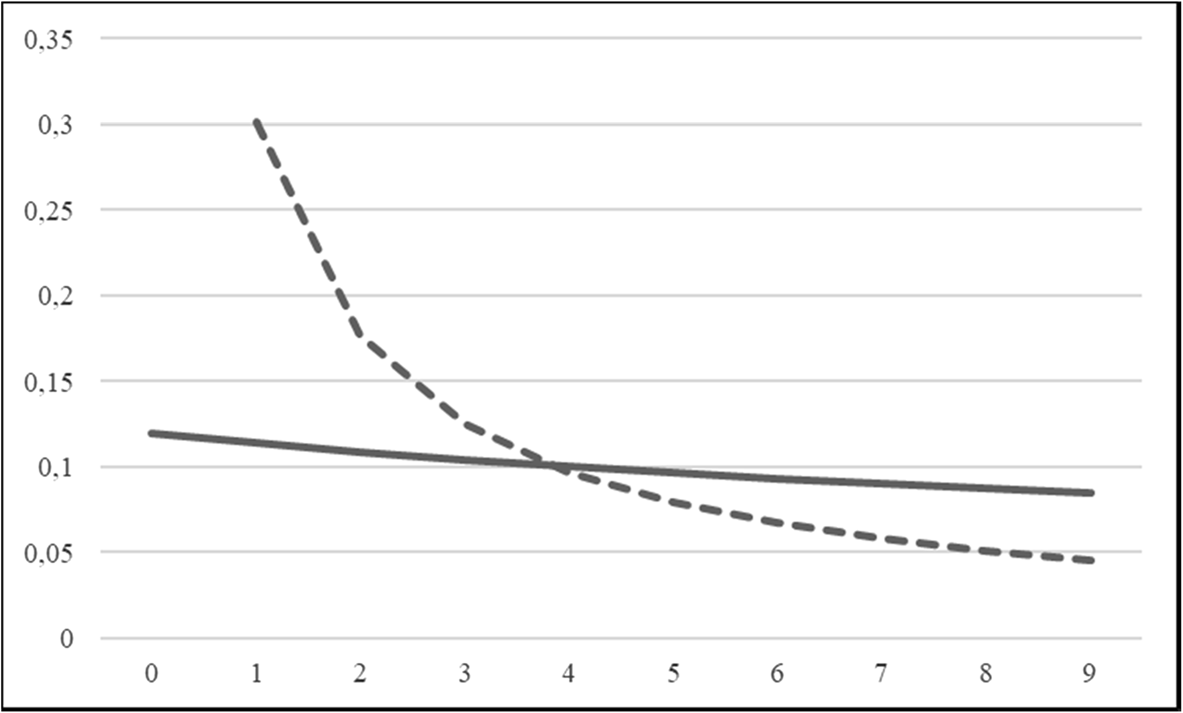
\includegraphics[width=\linewidth,height=0.6\textheight,keepaspectratio]{gfx/m2l4a_benford_fig1_expected_frequencies.png}
\par\smallskip{\small \textbf{Hình 1:} Tần số kỳ vọng của Benford cho chữ số thứ nhất và thứ hai.}
\end{figure}

Hình 1 Tần số kỳ vọng của Benford cho chữ số thứ nhất và thứ hai. Hình này chứa biểu diễn đồ họa của các tần số kỳ vọng cho chữ số thứ nhất (đường đứt nét) và cho chữ số thứ hai (đường liền nét) dựa trên phân phối của Benford. Các giá trị trên trục dọc là xác suất phân phối của chữ số $i$ như được hiển thị trên trục ngang, với $i=0, 1, 2, \ldots, 9$.

% [PDF p.9]
Bảng 2 Các biến kế toán ngân hàng và nguồn dữ liệu

{\small
\begin{longtable}{>{\raggedright\arraybackslash}p{0.198\linewidth}>{\raggedright\arraybackslash}p{0.481\linewidth}>{\raggedright\arraybackslash}p{0.117\linewidth}>{\raggedright\arraybackslash}p{0.144\linewidth}}
\toprule
\textbf{Thành phần CAMEL (CAMEL components)} & \textbf{Các biến số (Variables)} & \textbf{Ký hiệu (Abbreviation)} & \textbf{Nguồn dữ liệu (Data Source)} \\
\midrule
\endhead
Mức độ an toàn vốn (Capital adequacy) & Vốn pháp định cốt lõi (Core regulatory capital) & TIER1 & Báo cáo Call (Call reports) \\
\addlinespace[2pt]
 & Vốn chủ sở hữu theo sổ sách (Book equity capital) & EQUITY &  \\
\addlinespace[2pt]
Chất lượng tài sản (Asset quality) & Chi phí dự phòng tổn thất cho vay (Loan loss provisions) & LLP &  \\
\addlinespace[2pt]
 & Số dư dự phòng tổn thất cho vay (Allowances for loan losses) & ALLOW &  \\
\addlinespace[2pt]
 & Nợ xấu (Non-performing loans) & NPL &  \\
\addlinespace[2pt]
Sức mạnh thu nhập (Earnings strength) & Tổng thu nhập lãi (Total interest income) & INTINC &  \\
\addlinespace[2pt]
 & Tổng thu nhập ngoài lãi (Total non-interest income) & NINTINC &  \\
\addlinespace[2pt]
 & Tổng tài sản sinh lời (Total earning assets) & EARNAS &  \\
\addlinespace[2pt]
Tính thanh khoản (Liquidity) & Tiền mặt và số dư tại các tổ chức nhận tiền gửi (Cash and balances due from depository institutions) & CASH &  \\
\addlinespace[2pt]
 & Tiền mua quỹ liên bang và chứng khoán bán theo hợp đồng mua lại (Federal funds purchased and securities sold under agreements to repurchase) & REPOS &  \\
\addlinespace[2pt]
\bottomrule
\end{longtable}
}

Bảng này trình bày tất cả các biến số mà chúng tôi sử dụng trong phân tích thực nghiệm của mình. Ký hiệu của mỗi biến số và nguồn mà chúng tôi sử dụng để thu thập dữ liệu kế toán tương ứng cũng được báo cáo ở hai cột cuối cùng.

% [PDF p.11]
\begin{landscape}
{\small\textbf{Bảng 3} Phân tích chữ số ở vị trí thứ hai trong giai đoạn trước khủng hoảng\par}\smallskip
\begin{center}
{\tiny\setlength{\tabcolsep}{2pt}
\begin{adjustbox}{max width=\textheight}
\begin{tabular}{lcccccccccccccccc}
\toprule
\textbf{Chữ số (Digit)} & \textbf{\shortstack{Tần số kỳ vọng (Exp.\\freq.)}} & \textbf{\shortstack{TIER1\\Không kiệt quệ\\n=118,801\\Sai lệch quan sát\\(z-statistic)}} & \textbf{\shortstack{TIER1\\Phá sản\\n=8,036\\Sai lệch quan sát\\(z-statistic)}} & \textbf{\shortstack{TIER1\\Được cứu trợ\\n=14,918\\Sai lệch quan sát\\(z-statistic)}} & \textbf{\shortstack{LLP\\Không kiệt quệ\\n=116,805\\Sai lệch quan sát\\(z-statistic)}} & \textbf{\shortstack{LLP\\Phá sản\\n=7,633\\Sai lệch quan sát\\(z-statistic)}} & \textbf{\shortstack{LLP\\Được cứu trợ\\n=14,008\\Sai lệch quan sát\\(z-statistic)}} & \textbf{\shortstack{INTINC\\Không kiệt quệ\\n=119,382\\Sai lệch quan sát\\(z-statistic)}} & \textbf{\shortstack{INTINC\\Phá sản\\n=8,439\\Sai lệch quan sát\\(z-statistic)}} & \textbf{\shortstack{INTINC\\Được cứu trợ\\n=15,402\\Sai lệch quan sát\\(z-statistic)}} & \textbf{\shortstack{NINTINC\\Không kiệt quệ\\n=119,270\\Sai lệch quan sát\\(z-statistic)}} & \textbf{\shortstack{NINTINC\\Phá sản\\n=8,421\\Sai lệch quan sát\\(z-statistic)}} & \textbf{\shortstack{NINTINC\\Được cứu trợ\\n=15,426\\Sai lệch quan sát\\(z-statistic)}} & \textbf{\shortstack{CASH\\Không kiệt quệ\\n=119,320\\Sai lệch quan sát\\(z-statistic)}} & \textbf{\shortstack{CASH\\Phá sản\\n=8,296\\Sai lệch quan sát\\(z-statistic)}} & \textbf{\shortstack{CASH\\Được cứu trợ\\n=15,224\\Sai lệch quan sát\\(z-statistic)}} \\
\midrule
0 & .1197 & \shortstack{0.0147\\1.33} & \shortstack{0.0344\\1.20} & \shortstack{0.0272\\1.41} & \shortstack{-0.0414\\-1.87*} & \shortstack{-0.0571\\-1.99**} & \shortstack{-0.0793\\-2.09**} & \shortstack{0.0556\\2.30**} & \shortstack{0.0730\\2.41**} & \shortstack{0.0732\\2.69***} & \shortstack{0.0181\\1.39} & \shortstack{0.0182\\1.51} & \shortstack{0.0820\\2.34**} & \shortstack{-0.0032\\-0.84} & \shortstack{-0.0096\\-1.20} & \shortstack{0.0103\\0.54} \\
1 & .1139 & \shortstack{0.0115\\0.92} & \shortstack{0.0219\\1.43} & \shortstack{0.0238\\1.32} & \shortstack{-0.0208\\-1.30} & \shortstack{-0.0093\\-1.28} & \shortstack{-0.0094\\-1.55} & \shortstack{0.0395\\1.74*} & \shortstack{0.0476\\2.18**} & \shortstack{0.0390\\2.13**} & \shortstack{0.0116\\1.30} & \shortstack{0.0103\\0.96} & \shortstack{0.0346\\1.69*} & \shortstack{0.0029\\0.41} & \shortstack{-0.0042\\-1.02} & \shortstack{0.0087\\0.67} \\
2 & .1088 & \shortstack{-0.0028\\-1.10} & \shortstack{-0.0226\\-1.03} & \shortstack{0.0170\\1.21} & \shortstack{0.0122\\0.95} & \shortstack{0.0032\\1.17} & \shortstack{-0.0086\\-1.48} & \shortstack{-0.0192\\-1.10} & \shortstack{0.0202\\1.49} & \shortstack{0.0136\\1.22} & \shortstack{0.0042\\1.14} & \shortstack{0.0129\\1.17} & \shortstack{-0.0125\\-0.85} & \shortstack{0.0010\\0.23} & \shortstack{0.0053\\0.67} & \shortstack{-0.0094\\-1.05} \\
3 & .1043 & \shortstack{0.0023\\1.17} & \shortstack{-0.0094\\-0.89} & \shortstack{-0.0115\\-0.95} & \shortstack{0.0109\\0.67} & \shortstack{0.0014\\0.91} & \shortstack{0.0051\\1.04} & \shortstack{0.0153\\1.28} & \shortstack{-0.0218\\-1.10} & \shortstack{-0.0067\\-0.93} & \shortstack{-0.0049\\-0.95} & \shortstack{0.0002\\0.54} & \shortstack{-0.0062\\-0.68} & \shortstack{0.0004\\0.49} & \shortstack{0.0039\\0.78} & \shortstack{-0.0060\\-1.21} \\
4 & .1003 & \shortstack{0.0016\\0.68} & \shortstack{0.0048\\0.99} & \shortstack{0.0102\\1.18} & \shortstack{-0.0075\\-1.26} & \shortstack{-0.0010\\-0.73} & \shortstack{0.0019\\0.88} & \shortstack{0.0042\\1.13} & \shortstack{-0.0094\\-1.29} & \shortstack{-0.0051\\-1.17} & \shortstack{-0.0051\\-0.99} & \shortstack{0.0035\\0.70} & \shortstack{0.0035\\0.31} & \shortstack{-0.0029\\-0.58} & \shortstack{0.0008\\0.45} & \shortstack{0.0039\\0.50} \\
5 & .0967 & \shortstack{0.0014\\0.72} & \shortstack{0.0037\\1.06} & \shortstack{-0.0008\\-0.48} & \shortstack{-0.0053\\-1.18} & \shortstack{0.0009\\1.05} & \shortstack{-0.0012\\-0.76} & \shortstack{0.0039\\1.06} & \shortstack{0.0048\\0.85} & \shortstack{0.0021\\0.96} & \shortstack{-0.0004\\-1.17} & \shortstack{0.0032\\1.05} & \shortstack{0.0028\\0.63} & \shortstack{0.0012\\0.92} & \shortstack{0.0004\\1.12} & \shortstack{0.0021\\0.87} \\
6 & .0934 & \shortstack{-0.0022\\-0.58} & \shortstack{0.0032\\0.38} & \shortstack{0.0014\\1.07} & \shortstack{0.0061\\1.04} & \shortstack{-0.0018\\-0.63} & \shortstack{-0.0009\\-0.97} & \shortstack{0.0044\\1.02} & \shortstack{0.0032\\1.18} & \shortstack{-0.0048\\-1.00} & \shortstack{0.0013\\0.62} & \shortstack{0.0003\\0.64} & \shortstack{0.0022\\1.17} & \shortstack{0.0020\\1.04} & \shortstack{-0.0055\\-0.53} & \shortstack{-0.0009\\-1.04} \\
7 & .0904 & \shortstack{-0.0018\\-0.69} & \shortstack{-0.0029\\-1.15} & \shortstack{-0.0114\\-1.41} & \shortstack{0.0116\\1.17} & \shortstack{-0.0020\\-0.87} & \shortstack{0.0044\\1.29} & \shortstack{0.0098\\1.16} & \shortstack{-0.0097\\-1.39} & \shortstack{-0.0105\\-1.18} & \shortstack{-0.0040\\-1.16} & \shortstack{0.0095\\1.18} & \shortstack{-0.0173\\-1.29} & \shortstack{-0.0039\\-0.62} & \shortstack{-0.0126\\-1.10} & \shortstack{-0.0028\\-0.63} \\
8 & .0876 & \shortstack{-0.0130\\-1.14} & \shortstack{-0.0174\\-1.38} & \shortstack{-0.0249\\-1.38} & \shortstack{0.0125\\1.04} & \shortstack{0.0082\\1.38} & \shortstack{0.0084\\1.40} & \shortstack{-0.0256\\-2.05**} & \shortstack{-0.0425\\-2.28**} & \shortstack{-0.0342\\-1.79*} & \shortstack{-0.0032\\-1.03} & \shortstack{-0.0053\\-1.02} & \shortstack{-0.0259\\-1.84*} & \shortstack{-0.0040\\-0.51} & \shortstack{0.0153\\0.83} & \shortstack{0.0070\\1.38} \\
9 & .0850 & \shortstack{-0.0141\\-0.93} & \shortstack{-0.0351\\-1.49} & \shortstack{-0.0308\\-1.33} & \shortstack{0.0452\\1.98**} & \shortstack{0.0489\\1.94*} & \shortstack{0.0738\\2.32**} & \shortstack{-0.0718\\-2.26**} & \shortstack{-0.0822\\-2.49**} & \shortstack{-0.0816\\-2.55**} & \shortstack{-0.0053\\-1.40} & \shortstack{-0.0128\\-1.44} & \shortstack{-0.0782\\-2.41**} & \shortstack{-0.0103\\-1.02} & \shortstack{0.0188\\0.99} & \shortstack{0.0106\\0.92} \\
$\chi^2_{(9)}$ &  & 5.18 & 9.31 & 10.83 & 15.19* & 17.19** & 17.93** & 18.19** & 19.88** & 20.07** & 9.31 & 6.93 & 18.05*** & 5.30 & 2.76 & 3.58 \\
\bottomrule
\end{tabular}
\end{adjustbox}}
\end{center}
\end{landscape}

Cột đầu tiên của Bảng liệt kê tất cả mười chữ số có khả năng xuất hiện ở vị trí thứ hai của các biến số được kiểm tra, trong khi tần số xuất hiện kỳ vọng cho mỗi chữ số được xác định bởi Định luật Benford được trình bày ở cột thứ hai. Phần còn lại của các cột báo cáo các sai lệch quan sát được giữa tần số thực tế và kỳ vọng cho từng biến số (TIER1, LLP, INTINC, NINTINC, CASH) đối với các nhóm ngân hàng không bị kiệt quệ, phá sản, và được cứu trợ trong giai đoạn trước khủng hoảng. Giá trị của thống kê z và mức ý nghĩa tương ứng được trình bày bên dưới sai lệch quan sát được cho mỗi chữ số. Các giá trị của kiểm định mức độ phù hợp (goodness-of-fit) chi-bình phương được báo cáo ở hàng cuối cùng của Bảng. Tất cả các biến số và nguồn dữ liệu của chúng được mô tả trong Bảng 2. ***, **, và * chỉ ra ý nghĩa thống kê tương ứng ở mức 1\%, 5\%, và 10\%.

% [PDF p.12]
\begin{landscape}
{\small\textbf{Bảng 4} Phân tích chữ số ở vị trí thứ hai trong giai đoạn khủng hoảng\par}\smallskip
\begin{center}
{\tiny\setlength{\tabcolsep}{2pt}
\begin{adjustbox}{max width=\textheight}
\begin{tabular}{lccccccccccccc}
\toprule
\textbf{Chữ số (Digit)} & \textbf{\shortstack{Tần số kỳ vọng (Exp.\\freq.)}} & \textbf{\shortstack{TIER1\\Không kiệt quệ\\n=118,801\\Sai lệch quan sát\\(z-statistic)}} & \textbf{\shortstack{TIER1\\Phá sản\\n=8,036\\Sai lệch quan sát\\(z-statistic)}} & \textbf{\shortstack{TIER1\\Được cứu trợ\\n=14,918\\Sai lệch quan sát\\(z-statistic)}} & \textbf{\shortstack{LLP\\Không kiệt quệ\\n=116,805\\Sai lệch quan sát\\(z-statistic)}} & \textbf{\shortstack{LLP\\Phá sản\\n=7,633\\Sai lệch quan sát\\(z-statistic)}} & \textbf{\shortstack{LLP\\Được cứu trợ\\n=14,008\\Sai lệch quan sát\\(z-statistic)}} & \textbf{\shortstack{INTINC\\Không kiệt quệ\\n=119,382\\Sai lệch quan sát\\(z-statistic)}} & \textbf{\shortstack{INTINC\\Phá sản\\n=8,439\\Sai lệch quan sát\\(z-statistic)}} & \textbf{\shortstack{INTINC\\Được cứu trợ\\n=15,402\\Sai lệch quan sát\\(z-statistic)}} & \textbf{\shortstack{NINTINC\\Không kiệt quệ\\n=119,270\\Sai lệch quan sát\\(z-statistic)}} & \textbf{\shortstack{NINTINC\\Phá sản\\n=8,421\\Sai lệch quan sát\\(z-statistic)}} & \textbf{\shortstack{NINTINC\\Được cứu trợ\\n=15,426\\Sai lệch quan sát\\(z-statistic)}} \\
\midrule
0 & .1197 & \shortstack{0.0498\\5.89***} & \shortstack{0.0582\\7.41***} & \shortstack{0.0632\\8.09***} & \shortstack{-0.0582\\-3.85***} & \shortstack{-0.0692\\-4.98***} & \shortstack{-0.0882\\-7.53***} & \shortstack{0.0641\\5.12***} & \shortstack{0.0788\\8.75***} & \shortstack{0.0778\\6.93***} & \shortstack{0.0305\\-0.75} & \shortstack{0.0274\\1.39} & \shortstack{0.0873\\8.94***} \\
1 & .3010 & \shortstack{0.0271\\2.34**} & \shortstack{0.0263\\3.03***} & \shortstack{0.0305\\2.19**} & \shortstack{-0.0372\\-2.09**} & \shortstack{-0.0391\\-2.51**} & \shortstack{-0.0358\\-2.97***} & \shortstack{0.0531\\4.12***} & \shortstack{0.0496\\3.63***} & \shortstack{0.0484\\4.70***} & \shortstack{0.0019\\0.56} & \shortstack{0.0270\\0.74} & \shortstack{0.0396\\2.48**} \\
2 & .1761 & \shortstack{0.0005\\0.51} & \shortstack{0.0013\\0.64} & \shortstack{0.0009\\0.50} & \shortstack{0.0028\\0.53} & \shortstack{-0.0037\\-0.49} & \shortstack{-0.0005\\-0.64} & \shortstack{0.0103\\0.78} & \shortstack{0.0087\\0.56} & \shortstack{0.0112\\0.80} & \shortstack{0.0007\\0.41} & \shortstack{0.0012\\0.56} & \shortstack{0.0052\\0.48} \\
3 & .1249 & \shortstack{-0.0039\\-0.88} & \shortstack{-0.0028\\-0.92} & \shortstack{0.0018\\0.39} & \shortstack{0.0002\\0.90} & \shortstack{-0.0010\\-0.74} & \shortstack{0.0015\\0.55} & \shortstack{0.0032\\0.84} & \shortstack{0.0028\\1.18} & \shortstack{-0.0003\\-1.05} & \shortstack{0.0019\\0.72} & \shortstack{-0.0009\\-0.88} & \shortstack{0.0021\\0.27} \\
4 & .0969 & \shortstack{0.0026\\1.05} & \shortstack{-0.0032\\-0.84} & \shortstack{-0.0043\\-0.95} & \shortstack{0.0028\\0.49} & \shortstack{-0.0004\\-0.91} & \shortstack{-0.0018\\-1.18} & \shortstack{0.0006\\0.26} & \shortstack{0.0012\\0.38} & \shortstack{-0.0018\\-0.49} & \shortstack{-0.0002\\-1.12} & \shortstack{-0.0010\\-1.04} & \shortstack{0.0002\\0.69} \\
5 & .0792 & \shortstack{0.0009\\0.17} & \shortstack{-0.0013\\-0.28} & \shortstack{-0.0020\\-0.58} & \shortstack{0.0033\\0.89} & \shortstack{0.0014\\1.10} & \shortstack{-0.0028\\-0.65} & \shortstack{-0.0033\\-0.12} & \shortstack{-0.0030\\-0.19} & \shortstack{0.0012\\0.65} & \shortstack{0.0018\\0.33} & \shortstack{0.0041\\0.55} & \shortstack{-0.0010\\-0.70} \\
6 & .0670 & \shortstack{-0.0055\\-1.26} & \shortstack{0.0054\\0.98} & \shortstack{-0.0041\\-1.00} & \shortstack{0.0005\\0.59} & \shortstack{0.0011\\0.70} & \shortstack{-0.0017\\-0.81} & \shortstack{0.0003\\0.86} & \shortstack{0.0010\\0.88} & \shortstack{0.0015\\0.73} & \shortstack{0.0028\\1.03} & \shortstack{-0.0046\\-0.78} & \shortstack{0.0031\\0.98} \\
7 & .0580 & \shortstack{0.0083\\1.30} & \shortstack{0.0094\\1.29} & \shortstack{0.0102\\1.36} & \shortstack{-0.0037\\-0.83} & \shortstack{-0.0022\\-1.03} & \shortstack{0.0030\\0.94} & \shortstack{0.0041\\0.92} & \shortstack{0.0032\\1.03} & \shortstack{-0.0009\\-0.99} & \shortstack{0.0002\\0.88} & \shortstack{0.0021\\0.39} & \shortstack{-0.0072\\-1.34} \\
8 & .0512 & \shortstack{-0.0088\\-2.23**} & \shortstack{-0.0104\\-3.04***} & \shortstack{-0.0086\\-1.97**} & \shortstack{0.0051\\1.45} & \shortstack{0.0038\\1.20} & \shortstack{0.0047\\1.51} & \shortstack{-0.0196\\-4.83***} & \shortstack{-0.0185\\-2.56**} & \shortstack{-0.0163\\-2.71***} & \shortstack{0.0092\\0.67} & \shortstack{-0.0018\\-0.49} & \shortstack{-0.0103\\-1.99**} \\
9 & .0458 & \shortstack{-0.0201\\-2.04**} & \shortstack{-0.0185\\-2.18**} & \shortstack{-0.0240\\-2.69***} & \shortstack{0.0387\\2.37**} & \shortstack{0.0379\\2.27**} & \shortstack{0.0354\\3.17***} & \shortstack{-0.0316\\-5.31***} & \shortstack{-0.0302\\-2.48**} & \shortstack{-0.0289\\-2.95***} & \shortstack{-0.0018\\-0.74} & \shortstack{-0.0006\\-0.99} & \shortstack{-0.0304\\-3.05***} \\
$\chi^2_{(9)}$ &  & 20.05** & 24.09*** & 18.44** & 17.38** & 19.27** & 25.07*** & 23.21*** & 18.52** & 24.61*** & 8.12 & 7.10 & 19.28** \\
\bottomrule
\end{tabular}
\end{adjustbox}}
\end{center}
\end{landscape}

Cột đầu tiên của Bảng liệt kê tất cả mười chữ số có khả năng xuất hiện ở vị trí thứ hai của các biến số được kiểm tra, trong khi tần số xuất hiện kỳ vọng cho mỗi chữ số được xác định bởi Định luật Benford được trình bày ở cột thứ hai. Phần còn lại của các cột báo cáo các sai lệch quan sát được giữa tần số thực tế và kỳ vọng cho từng biến số (TIER1, LLP, INTINC, NINTINC, CASH) đối với các nhóm ngân hàng không bị kiệt quệ, phá sản, và được cứu trợ trong giai đoạn khủng hoảng. Giá trị của thống kê z và mức ý nghĩa tương ứng được trình bày bên dưới sai lệch quan sát được cho mỗi chữ số. Các giá trị của kiểm định mức độ phù hợp (goodness-of-fit) chi-bình phương được báo cáo ở hàng cuối cùng của Bảng. Tất cả các biến số và nguồn dữ liệu của chúng được mô tả trong Bảng 2. ***, **, và * chỉ ra ý nghĩa thống kê tương ứng ở mức 1\%, 5\%, và 10\%.

% [PDF p.13 | Hình 2, chú thích ở PDF p.14]
\begin{figure}[H]
\centering
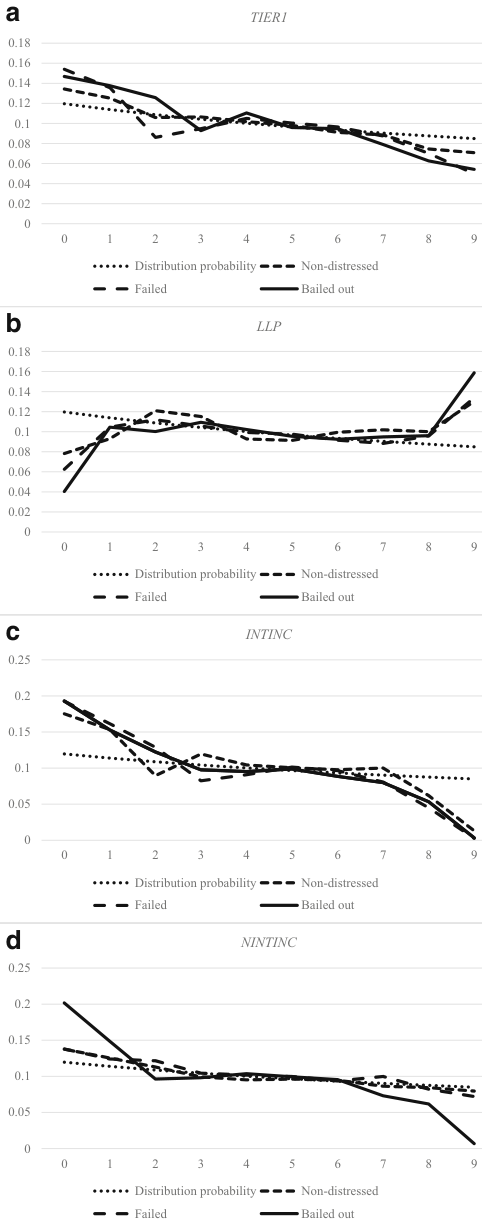
\includegraphics[width=\linewidth,height=0.6\textheight,keepaspectratio]{gfx/m2l4a_benford_fig2_pre_crisis_second_digit.png}
\par\smallskip{\small \textbf{Hình 2:} Biểu diễn đồ họa kết quả phân tích chữ số trong giai đoạn trước khủng hoảng.}
\end{figure}

Hình 2 Biểu diễn đồ họa kết quả phân tích chữ số trong giai đoạn trước khủng hoảng. Các Panel A, B, C và D cung cấp biểu diễn đồ họa kết quả phân tích chữ số ở vị trí thứ hai của các biến kế toán bị thao túng (lần lượt là \emph{TIER1}, \emph{LLP}, \emph{INTINC} và \emph{NINTINC}) trong giai đoạn trước khủng hoảng. Các giá trị trên trục dọc là xác suất phân phối của chữ số $i$ ($i=0, 1, 2, \ldots, 9$) như hiển thị trên trục ngang.

% [PDF p.15 | Hình 3, chú thích ở PDF p.16]
\begin{figure}[H]
\centering
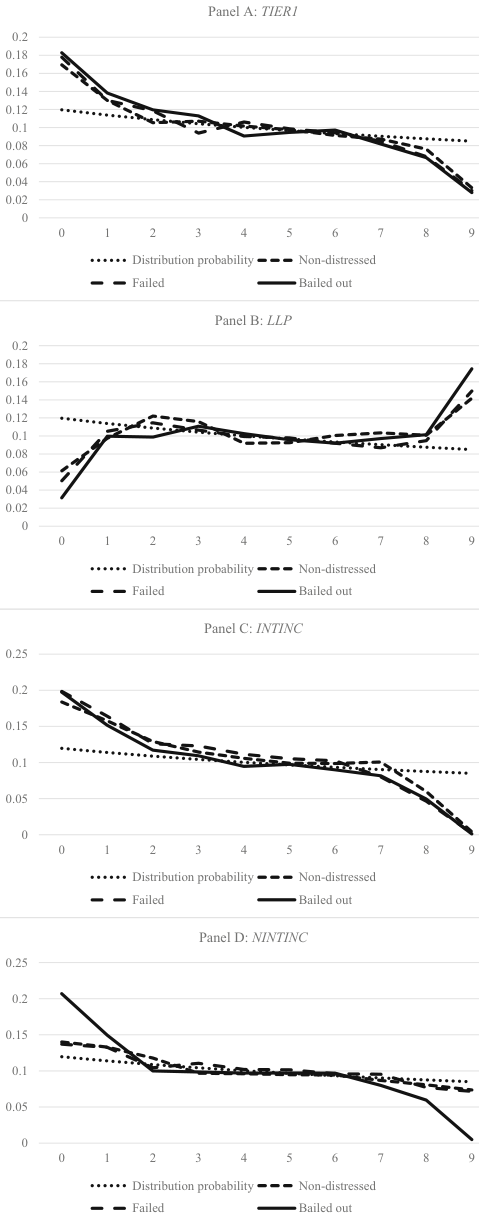
\includegraphics[width=\linewidth,height=0.6\textheight,keepaspectratio]{gfx/m2l4a_benford_fig3_crisis_second_digit.png}
\par\smallskip{\small \textbf{Hình 3:} Biểu diễn đồ họa kết quả phân tích chữ số trong giai đoạn khủng hoảng.}
\end{figure}

Hình 3 Biểu diễn đồ họa kết quả phân tích chữ số trong giai đoạn khủng hoảng. Các Panel A, B, C và D cung cấp biểu diễn đồ họa kết quả phân tích chữ số ở vị trí thứ hai của các biến kế toán bị thao túng (lần lượt là \emph{TIER1}, \emph{LLP}, \emph{INTINC} và \emph{NINTINC}) trong giai đoạn khủng hoảng. Các giá trị trên trục dọc là xác suất phân phối của chữ số $i$ ($i=0, 1, 2, \ldots, 9$) như hiển thị trên trục ngang.

% [PDF p.17]
Bảng 5 Ý nghĩa thống kê của các sai lệch được báo cáo so với Định luật Benford đối với chữ số không

{\small
\begin{longtable}{>{\raggedright\arraybackslash}p{0.329\linewidth}>{\raggedright\arraybackslash}p{0.172\linewidth}>{\raggedright\arraybackslash}p{0.135\linewidth}>{\raggedright\arraybackslash}p{0.304\linewidth}}
\toprule
\textbf{} & \textbf{Giai đoạn trước khủng hoảng (Pre-crisis\newline{}period)} & \textbf{Giai đoạn khủng hoảng (Crisis\newline{}period)} & \textbf{Giai đoạn trước khủng hoảng so với Khủng hoảng (Pre-crisis vs Crisis\newline{}(z-statistic))} \\
\midrule
\endhead
\emph{\textbf{Panel A: TIER1}} &  &  &  \\
\addlinespace[2pt]
\textbf{Các ngân hàng không bị kiệt quệ (Non-distressed banks)} & 0.0147 & 0.0498 & 1.98** \\
\addlinespace[2pt]
\textbf{Các ngân hàng phá sản (Failed banks)} & 0.0344 & 0.0582 & 2.60*** \\
\addlinespace[2pt]
\textbf{Các ngân hàng được cứu trợ (Bailed-out banks)} & 0.0272 & 0.0632 & 2.91*** \\
\addlinespace[2pt]
Các ngân hàng không bị kiệt quệ so với phá sản (Non-distressed vs Failed banks\newline{}(z-statistic)) & 1.24 & 2.02** &  \\
\addlinespace[2pt]
Các ngân hàng không bị kiệt quệ so với được cứu trợ (Non-distressed vs Bailed-out banks\newline{}(z-statistic)) & 1.06 & 2.33** &  \\
\addlinespace[2pt]
Các ngân hàng phá sản so với được cứu trợ (Failed vs Bailed-out banks\newline{}(z-statistic)) & 0.87 & 1.14 &  \\
\addlinespace[2pt]
\emph{\textbf{Panel B: LLP}} &  &  &  \\
\addlinespace[2pt]
\textbf{Các ngân hàng không bị kiệt quệ (Non-distressed banks)} & -0.0414 & -0.0582 & -2.05** \\
\addlinespace[2pt]
\textbf{Các ngân hàng phá sản (Failed banks)} & -0.0571 & -0.0692 & -2.31** \\
\addlinespace[2pt]
\textbf{Các ngân hàng được cứu trợ (Bailed-out banks)} & -0.0793 & -0.0882 & -2.88*** \\
\addlinespace[2pt]
Các ngân hàng không bị kiệt quệ so với phá sản (Non-distressed vs Failed banks\newline{}(z-statistic)) & -1.99** & -2.10** &  \\
\addlinespace[2pt]
Các ngân hàng không bị kiệt quệ so với được cứu trợ (Non-distressed vs Bailed-out banks\newline{}(z-statistic)) & -2.24** & -2.23** &  \\
\addlinespace[2pt]
Các ngân hàng phá sản so với được cứu trợ (Failed vs Bailed-out banks\newline{}(z-statistic)) & -0.90 & -0.82 &  \\
\addlinespace[2pt]
\emph{\textbf{Panel C: INTINC}} &  &  &  \\
\addlinespace[2pt]
\textbf{Các ngân hàng không bị kiệt quệ (Non-distressed banks)} & 0.0556 & 0.0641 & 2.19** \\
\addlinespace[2pt]
\textbf{Các ngân hàng phá sản (Failed banks)} & 0.0730 & 0.0788 & 2.02** \\
\addlinespace[2pt]
\textbf{Các ngân hàng được cứu trợ (Bailed-out banks)} & 0.0732 & 0.0778 & 2.31** \\
\addlinespace[2pt]
Các ngân hàng không bị kiệt quệ so với phá sản (Non-distressed vs Failed banks\newline{}(z-statistic)) & 2.10** & 1.99** &  \\
\addlinespace[2pt]
Các ngân hàng không bị kiệt quệ so với được cứu trợ (Non-distressed vs Bailed-out banks\newline{}(z-statistic)) & 2.24** & 2.06** &  \\
\addlinespace[2pt]
Các ngân hàng phá sản so với được cứu trợ (Failed vs Bailed-out banks\newline{}(z-statistic)) & 1.38 & 1.40 &  \\
\addlinespace[2pt]
\emph{\textbf{Panel D: NINTINC}} &  &  &  \\
\addlinespace[2pt]
\textbf{Các ngân hàng không bị kiệt quệ (Non-distressed banks)} & 0.0281 & 0.0305 & 0.93 \\
\addlinespace[2pt]
\textbf{Các ngân hàng phá sản (Failed banks)} & 0.0382 & 0.0274 & 1.05 \\
\addlinespace[2pt]
\textbf{Các ngân hàng được cứu trợ (Bailed-out banks)} & 0.0820 & 0.0873 & 2.09** \\
\addlinespace[2pt]
Các ngân hàng không bị kiệt quệ so với phá sản (Non-distressed vs Failed banks\newline{}(z-statistic)) & 1.14 & 1.07 &  \\
\addlinespace[2pt]
Các ngân hàng không bị kiệt quệ so với được cứu trợ (Non-distressed vs Bailed-out banks\newline{}(z-statistic)) & 3.95*** & 4.11*** &  \\
\addlinespace[2pt]
Các ngân hàng phá sản so với được cứu trợ (Failed vs Bailed-out banks\newline{}(z-statistic)) & 2.44** & 2.70*** &  \\
\addlinespace[2pt]
\bottomrule
\end{longtable}
}

Bảng này trình bày các sai lệch so với Định luật Benford đối với chữ số không giữa ba loại hình ngân hàng (các ngân hàng không bị kiệt quệ, phá sản, và được cứu trợ) và trong hai giai đoạn thời gian đối với bốn biến số (TIER1, LLP, INTINC, NINTINC) được phát hiện là bị thao túng trong phân tích cơ sở của chúng tôi. Các giá trị của các kiểm định ý nghĩa thống kê liên quan dựa trên thống kê z cũng được báo cáo. Tất cả các biến số và nguồn dữ liệu của chúng được mô tả trong Bảng 2. ***, **, và * chỉ ra ý nghĩa thống kê tương ứng ở mức 1\%, 5\%, và 10\%.

% [PDF p.19]
\begin{landscape}
{\small\textbf{Bảng 6} Phân tích chữ số ở vị trí thứ nhất trong giai đoạn trước khủng hoảng\par}\smallskip
\begin{center}
{\tiny\setlength{\tabcolsep}{2pt}
\begin{adjustbox}{max width=\textheight}
\begin{tabular}{lcccccccccccccccc}
\toprule
\textbf{Chữ số (Digit)} & \textbf{\shortstack{Tần số kỳ vọng (Exp.\\freq.)}} & \textbf{\shortstack{TIER1\\Không kiệt quệ\\n=130,924\\Sai lệch quan sát\\(z-statistic)}} & \textbf{\shortstack{TIER1\\Phá sản\\n=9,093\\Sai lệch quan sát\\(z-statistic)}} & \textbf{\shortstack{TIER1\\Được cứu trợ\\n=16,690\\Sai lệch quan sát\\(z-statistic)}} & \textbf{\shortstack{LLP\\Không kiệt quệ\\n=130,337\\Sai lệch quan sát\\(z-statistic)}} & \textbf{\shortstack{LLP\\Phá sản\\n=8,792\\Sai lệch quan sát\\(z-statistic)}} & \textbf{\shortstack{LLP\\Được cứu trợ\\n=15,973\\Sai lệch quan sát\\(z-statistic)}} & \textbf{\shortstack{INTINC\\Không kiệt quệ\\n=131,527\\Sai lệch quan sát\\(z-statistic)}} & \textbf{\shortstack{INTINC\\Phá sản\\n=9,361\\Sai lệch quan sát\\(z-statistic)}} & \textbf{\shortstack{INTINC\\Được cứu trợ\\n=17,190\\Sai lệch quan sát\\(z-statistic)}} & \textbf{\shortstack{NINTINC\\Không kiệt quệ\\n=131,534\\Sai lệch quan sát\\(z-statistic)}} & \textbf{\shortstack{NINTINC\\Phá sản\\n=9,340\\Sai lệch quan sát\\(z-statistic)}} & \textbf{\shortstack{NINTINC\\Được cứu trợ\\n=17,118\\Sai lệch quan sát\\(z-statistic)}} & \textbf{\shortstack{CASH\\Không kiệt quệ\\n=131,429\\Sai lệch quan sát\\(z-statistic)}} & \textbf{\shortstack{CASH\\Phá sản\\n=9,305\\Sai lệch quan sát\\(z-statistic)}} & \textbf{\shortstack{CASH\\Được cứu trợ\\n=12,345\\Sai lệch quan sát\\(z-statistic)}} \\
\midrule
1 & .3010 & \shortstack{0.0498\\1.93*} & \shortstack{0.0582\\2.05**} & \shortstack{0.0652\\1.75*} & \shortstack{-0.0582\\-2.12**} & \shortstack{-0.0692\\-2.36**} & \shortstack{-0.0882\\-2.31**} & \shortstack{0.0641\\2.69***} & \shortstack{0.0788\\3.29***} & \shortstack{0.0778\\3.15***} & \shortstack{0.0205\\1.44} & \shortstack{0.0174\\1.39} & \shortstack{0.0873\\2.41**} & \shortstack{-0.0041\\-1.05} & \shortstack{-0.0082\\-0.78} & \shortstack{0.0079\\1.15} \\
2 & .1761 & \shortstack{0.0162\\1.42} & \shortstack{0.0163\\1.51} & \shortstack{0.0244\\1.41} & \shortstack{-0.0164\\-1.55} & \shortstack{-0.0087\\-0.96} & \shortstack{-0.0142\\-1.24} & \shortstack{0.0438\\1.85*} & \shortstack{0.0502\\2.31**} & \shortstack{0.0376\\2.34**} & \shortstack{0.0192\\1.40} & \shortstack{0.0188\\1.20} & \shortstack{0.0355\\2.06**} & \shortstack{0.0037\\0.56} & \shortstack{-0.0055\\-0.89} & \shortstack{0.0053\\1.02} \\
3 & .1249 & \shortstack{-0.0034\\-1.03} & \shortstack{0.0098\\0.65} & \shortstack{0.0109\\0.94} & \shortstack{0.0133\\1.14} & \shortstack{0.0058\\0.89} & \shortstack{-0.0100\\-1.38} & \shortstack{0.0203\\1.25} & \shortstack{0.0173\\1.30} & \shortstack{0.0083\\1.36} & \shortstack{0.0091\\0.89} & \shortstack{-0.0044\\-0.96} & \shortstack{-0.0089\\-1.04} & \shortstack{0.0048\\0.39} & \shortstack{0.0040\\1.04} & \shortstack{-0.0067\\-0.38} \\
4 & .0969 & \shortstack{0.0028\\0.95} & \shortstack{-0.0104\\-1.12} & \shortstack{0.0086\\1.23} & \shortstack{0.0117\\0.81} & \shortstack{0.0023\\1.02} & \shortstack{0.0065\\0.78} & \shortstack{0.0102\\0.97} & \shortstack{0.0187\\0.86} & \shortstack{0.0050\\0.31} & \shortstack{-0.0074\\-1.04} & \shortstack{0.0063\\0.69} & \shortstack{-0.0058\\-0.96} & \shortstack{0.0009\\0.56} & \shortstack{0.0027\\1.18} & \shortstack{-0.0050\\-0.59} \\
5 & .0792 & \shortstack{0.0014\\0.74} & \shortstack{0.0059\\0.75} & \shortstack{-0.0097\\-0.82} & \shortstack{-0.0084\\-1.18} & \shortstack{-0.0009\\-1.01} & \shortstack{0.0023\\0.59} & \shortstack{0.0056\\1.28} & \shortstack{0.0112\\0.68} & \shortstack{-0.0057\\-0.71} & \shortstack{-0.0042\\-0.73} & \shortstack{0.0018\\1.07} & \shortstack{-0.0033\\-0.40} & \shortstack{-0.0017\\-0.70} & \shortstack{0.0013\\0.64} & \shortstack{0.0018\\0.68} \\
6 & .0670 & \shortstack{0.0010\\0.83} & \shortstack{0.0020\\0.97} & \shortstack{-0.0021\\-0.33} & \shortstack{-0.0041\\-0.94} & \shortstack{0.0012\\0.87} & \shortstack{-0.0009\\-1.03} & \shortstack{0.0024\\1.10} & \shortstack{0.0086\\1.03} & \shortstack{0.0007\\1.26} & \shortstack{-0.0019\\-0.67} & \shortstack{0.0049\\0.61} & \shortstack{0.0004\\1.28} & \shortstack{0.0008\\1.02} & \shortstack{0.0010\\0.89} & \shortstack{0.0010\\1.05} \\
7 & .0580 & \shortstack{-0.0020\\-0.65} & \shortstack{0.0009\\0.59} & \shortstack{0.0038\\0.70} & \shortstack{0.0072\\1.19} & \shortstack{-0.0034\\-1.09} & \shortstack{-0.0014\\-1.12} & \shortstack{0.0052\\0.79} & \shortstack{0.0090\\0.78} & \shortstack{-0.0035\\-1.04} & \shortstack{0.0010\\0.77} & \shortstack{0.0028\\0.99} & \shortstack{0.0035\\0.49} & \shortstack{0.0033\\0.87} & \shortstack{-0.0101\\-1.19} & \shortstack{-0.0006\\-0.82} \\
8 & .0512 & \shortstack{-0.0031\\-0.88} & \shortstack{-0.0055\\-1.01} & \shortstack{-0.0085\\-1.05} & \shortstack{0.0131\\0.94} & \shortstack{-0.0034\\-1.15} & \shortstack{0.0068\\1.17} & \shortstack{0.0104\\0.83} & \shortstack{-0.0102\\-1.24} & \shortstack{-0.0087\\-0.96} & \shortstack{-0.0035\\-0.82} & \shortstack{0.0051\\0.52} & \shortstack{-0.0104\\-1.33} & \shortstack{-0.0028\\-0.54} & \shortstack{-0.0092\\-0.85} & \shortstack{-0.0021\\-0.78} \\
9 & .0458 & \shortstack{-0.0114\\-1.29} & \shortstack{-0.0198\\-1.49} & \shortstack{-0.0209\\-1.46} & \shortstack{0.0133\\1.47} & \shortstack{0.0073\\1.40} & \shortstack{0.0138\\1.32} & \shortstack{-0.0278\\-1.76*} & \shortstack{-0.0412\\-2.36**} & \shortstack{-0.0382\\-1.97**} & \shortstack{-0.0068\\-1.16} & \shortstack{-0.0104\\-1.21} & \shortstack{-0.0280\\-2.24**} & \shortstack{-0.0052\\-0.69} & \shortstack{0.0122\\1.06} & \shortstack{0.0064\\1.20} \\
$\chi^2_{(9)}$ &  & 14.93* & 16.98** & 15.11* & 17.56** & 19.25*** & 19.81** & 19.95** & 24.39*** & 23.17*** & 9.60 & 5.80 & 22.70*** & 6.18 & 4.29 & 5.07 \\
\bottomrule
\end{tabular}
\end{adjustbox}}
\end{center}
\end{landscape}

Cột đầu tiên của Bảng liệt kê các chữ số có khả năng xuất hiện ở vị trí thứ nhất của các biến số được kiểm tra, trong khi tần số xuất hiện kỳ vọng cho mỗi chữ số được xác định bởi Định luật Benford được trình bày ở cột thứ hai. Phần còn lại của các cột báo cáo các sai lệch quan sát được giữa tần số thực tế và kỳ vọng cho từng biến số (TIER1, LLP, INTINC, NINTINC, CASH) đối với các nhóm ngân hàng không bị kiệt quệ, phá sản, và được cứu trợ trong giai đoạn trước khủng hoảng. Giá trị của thống kê z và mức ý nghĩa tương ứng được trình bày bên dưới sai lệch quan sát được cho mỗi chữ số. Các giá trị của kiểm định mức độ phù hợp (goodness-of-fit) chi-bình phương được báo cáo ở hàng cuối cùng của Bảng. Tất cả các biến số và nguồn dữ liệu của chúng được mô tả trong Bảng 2. ***, **, và * chỉ ra ý nghĩa thống kê tương ứng ở mức 1\%, 5\%, và 10\%.

% [PDF p.21]
\begin{landscape}
{\small\textbf{Bảng 7} Kiểm tra tính vững: Phân tích chữ số ở vị trí thứ hai trong giai đoạn trước khủng hoảng\par}\smallskip
\begin{center}
{\tiny\setlength{\tabcolsep}{2pt}
\begin{adjustbox}{max width=\textheight}
\begin{tabular}{lcccccccccccccccc}
\toprule
\textbf{Chữ số (Digit)} & \textbf{\shortstack{Tần số kỳ vọng (Exp.\\freq.)}} & \textbf{\shortstack{EQUITY\\Không kiệt quệ\\n=118,939\\Sai lệch quan sát\\(z-statistic)}} & \textbf{\shortstack{EQUITY\\Phá sản\\n=8,190\\Sai lệch quan sát\\(z-statistic)}} & \textbf{\shortstack{EQUITY\\Được cứu trợ\\n=14,830\\Sai lệch quan sát\\(z-statistic)}} & \textbf{\shortstack{NPL\\Không kiệt quệ\\n=117,592\\Sai lệch quan sát\\(z-statistic)}} & \textbf{\shortstack{NPL\\Phá sản\\n=7,592\\Sai lệch quan sát\\(z-statistic)}} & \textbf{\shortstack{NPL\\Được cứu trợ\\n=14,142\\Sai lệch quan sát\\(z-statistic)}} & \textbf{\shortstack{ALLOW\\Không kiệt quệ\\n=118,671\\Sai lệch quan sát\\(z-statistic)}} & \textbf{\shortstack{ALLOW\\Phá sản\\n=7,920\\Sai lệch quan sát\\(z-statistic)}} & \textbf{\shortstack{ALLOW\\Được cứu trợ\\n=14,721\\Sai lệch quan sát\\(z-statistic)}} & \textbf{\shortstack{EARNAS\\Không kiệt quệ\\n=119,265\\Sai lệch quan sát\\(z-statistic)}} & \textbf{\shortstack{EARNAS\\Phá sản\\n=8,328\\Sai lệch quan sát\\(z-statistic)}} & \textbf{\shortstack{EARNAS\\Được cứu trợ\\n=15,275\\Sai lệch quan sát\\(z-statistic)}} & \textbf{\shortstack{REPOS\\Không kiệt quệ\\n=116,846\\Sai lệch quan sát\\(z-statistic)}} & \textbf{\shortstack{REPOS\\Phá sản\\n=7,146\\Sai lệch quan sát\\(z-statistic)}} & \textbf{\shortstack{REPOS\\Được cứu trợ\\n=13,951\\Sai lệch quan sát\\(z-statistic)}} \\
\midrule
0 & .1197 & \shortstack{0.0031\\0.44} & \shortstack{0.0163\\1.04} & \shortstack{0.0176\\1.34} & \shortstack{-0.0105\\-1.28} & \shortstack{-0.0310\\-1.33} & \shortstack{-0.0352\\-1.20} & \shortstack{-0.0053\\-0.85} & \shortstack{-0.0682\\-2.31**} & \shortstack{-0.0662\\-2.14**} & \shortstack{0.0488\\2.08**} & \shortstack{0.0632\\2.12**} & \shortstack{0.0671\\2.39**} & \shortstack{0.0040\\0.49} & \shortstack{0.0184\\1.03} & \shortstack{0.0081\\1.16} \\
1 & .1139 & \shortstack{0.0021\\0.49} & \shortstack{0.0103\\1.11} & \shortstack{0.0098\\1.17} & \shortstack{-0.0074\\-1.12} & \shortstack{-0.0206\\-1.42} & \shortstack{-0.0198\\-1.31} & \shortstack{0.0046\\0.94} & \shortstack{-0.0201\\-1.44} & \shortstack{-0.0170\\-1.38} & \shortstack{0.0374\\1.98**} & \shortstack{0.0459\\2.05**} & \shortstack{0.0391\\1.73*} & \shortstack{-0.0038\\-0.62} & \shortstack{0.0128\\1.21} & \shortstack{0.0052\\1.05} \\
2 & .1088 & \shortstack{0.0014\\0.36} & \shortstack{0.0053\\1.16} & \shortstack{0.0072\\1.23} & \shortstack{0.0079\\1.18} & \shortstack{-0.0131\\-1.20} & \shortstack{-0.0149\\-1.28} & \shortstack{-0.0037\\-1.08} & \shortstack{-0.0130\\-1.39} & \shortstack{-0.0094\\-1.56} & \shortstack{0.0137\\1.39} & \shortstack{0.0208\\1.43} & \shortstack{0.0157\\1.31} & \shortstack{-0.0022\\-0.48} & \shortstack{-0.0094\\-0.52} & \shortstack{0.0027\\0.43} \\
3 & .1043 & \shortstack{-0.0052\\-0.60} & \shortstack{0.0031\\0.94} & \shortstack{-0.0041\\-0.84} & \shortstack{0.0061\\1.05} & \shortstack{0.0127\\1.29} & \shortstack{-0.0102\\-0.95} & \shortstack{-0.0044\\-1.08} & \shortstack{0.0083\\1.32} & \shortstack{-0.0062\\-0.49} & \shortstack{-0.0125\\-1.20} & \shortstack{0.0121\\1.29} & \shortstack{-0.0059\\-1.33} & \shortstack{0.0020\\0.93} & \shortstack{-0.0048\\-0.71} & \shortstack{-0.0034\\-0.87} \\
4 & .1003 & \shortstack{-0.0023\\-0.37} & \shortstack{-0.0023\\-0.99} & \shortstack{-0.0031\\-0.99} & \shortstack{0.0053\\0.95} & \shortstack{0.0114\\0.69} & \shortstack{0.0061\\0.86} & \shortstack{-0.0035\\-1.14} & \shortstack{0.0057\\1.20} & \shortstack{0.0027\\0.83} & \shortstack{-0.0108\\-1.19} & \shortstack{-0.0054\\-1.38} & \shortstack{-0.0038\\-0.61} & \shortstack{0.0014\\0.61} & \shortstack{0.0016\\0.34} & \shortstack{-0.0028\\-1.16} \\
5 & .0967 & \shortstack{0.0019\\0.43} & \shortstack{-0.0014\\-1.18} & \shortstack{-0.0022\\-1.05} & \shortstack{-0.0054\\-1.02} & \shortstack{0.0086\\0.43} & \shortstack{0.0048\\0.22} & \shortstack{-0.0023\\-0.85} & \shortstack{-0.0021\\-0.95} & \shortstack{-0.0017\\-1.14} & \shortstack{0.0095\\0.98} & \shortstack{-0.0032\\-0.76} & \shortstack{-0.0021\\-0.83} & \shortstack{0.0008\\0.42} & \shortstack{0.0003\\1.10} & \shortstack{0.0032\\1.37} \\
6 & .0934 & \shortstack{0.0030\\0.61} & \shortstack{0.0020\\0.43} & \shortstack{0.0084\\0.59} & \shortstack{-0.0069\\-0.93} & \shortstack{0.0140\\-0.53} & \shortstack{0.0031\\1.05} & \shortstack{0.0057\\1.11} & \shortstack{0.0019\\1.36} & \shortstack{-0.0011\\-1.23} & \shortstack{0.0084\\0.69} & \shortstack{0.0048\\1.02} & \shortstack{0.0015\\1.25} & \shortstack{0.0004\\0.67} & \shortstack{-0.0011\\-0.74} & \shortstack{0.0039\\1.41} \\
7 & .0904 & \shortstack{-0.0039\\-0.28} & \shortstack{0.0038\\0.75} & \shortstack{0.0096\\1.14} & \shortstack{0.0089\\1.05} & \shortstack{0.0101\\1.18} & \shortstack{-0.0101\\-0.74} & \shortstack{0.0096\\1.08} & \shortstack{0.0203\\1.16} & \shortstack{0.0119\\1.30} & \shortstack{-0.0083\\-1.15} & \shortstack{-0.0105\\-1.38} & \shortstack{-0.0116\\-1.30} & \shortstack{-0.0014\\-1.02} & \shortstack{0.0040\\1.32} & \shortstack{0.0047\\0.78} \\
8 & .0876 & \shortstack{-0.0045\\-0.44} & \shortstack{0.0096\\1.09} & \shortstack{0.0101\\0.78} & \shortstack{0.0094\\1.07} & \shortstack{0.0232\\1.39} & \shortstack{0.0160\\1.41} & \shortstack{0.0129\\0.64} & \shortstack{0.0241\\1.54} & \shortstack{0.0284\\1.27} & \shortstack{-0.0264\\-1.76*} & \shortstack{-0.0319\\-1.84*} & \shortstack{-0.0261\\-1.78*} & \shortstack{-0.0027\\-0.94} & \shortstack{0.0111\\1.29} & \shortstack{-0.0109\\-1.11} \\
9 & .0850 & \shortstack{0.0059\\0.33} & \shortstack{-0.0149\\-0.85} & \shortstack{0.0126\\1.30} & \shortstack{0.0101\\1.18} & \shortstack{0.0288\\1.51} & \shortstack{0.0387\\1.44} & \shortstack{0.0148\\1.22} & \shortstack{0.0574\\2.43**} & \shortstack{0.0620\\2.49**} & \shortstack{-0.0608\\-2.31**} & \shortstack{-0.0841\\-2.34**} & \shortstack{-0.0858\\-2.36**} & \shortstack{-0.0049\\-0.88} & \shortstack{0.0173\\0.42} & \shortstack{-0.0125\\-0.94} \\
$\chi^2(9)$ &  & 2.49 & 4.62 & 3.19 & 4.93 & 10.74 & 9.17 & 6.09 & 18.34** & 17.55** & 17.48** & 18.94** & 17.27** & 2.90 & 2.62 & 4.01 \\
\bottomrule
\end{tabular}
\end{adjustbox}}
\end{center}
\end{landscape}

Cột đầu tiên của Bảng liệt kê tất cả mười chữ số có khả năng xuất hiện ở vị trí thứ hai của các biến số được kiểm tra, trong khi tần số xuất hiện kỳ vọng cho mỗi chữ số được xác định bởi Định luật Benford được trình bày ở cột thứ hai. Phần còn lại của các cột báo cáo các sai lệch quan sát được giữa tần số thực tế và kỳ vọng cho từng biến số (EQUITY, NPL, ALLOW, EARNAS, REPOS) đối với các nhóm ngân hàng không bị kiệt quệ, phá sản, và được cứu trợ trong giai đoạn trước khủng hoảng. Giá trị của thống kê z và mức ý nghĩa tương ứng được trình bày bên dưới sai lệch quan sát được cho mỗi chữ số. Các giá trị của kiểm định mức độ phù hợp (goodness-of-fit) chi-bình phương được báo cáo ở hàng cuối cùng của Bảng. Tất cả các biến số và nguồn dữ liệu của chúng được mô tả trong Bảng 2. ***, **, và * chỉ ra ý nghĩa thống kê tương ứng ở mức 1\%, 5\%, và 10\%.

% [PDF p.22]
\begin{landscape}
{\small\textbf{Bảng 8} Kiểm tra tính vững: Phân tích chữ số ở vị trí thứ hai trong giai đoạn khủng hoảng\par}\smallskip
\begin{center}
{\tiny\setlength{\tabcolsep}{2pt}
\begin{adjustbox}{max width=\textheight}
\begin{tabular}{lcccccccccccccccc}
\toprule
\textbf{Chữ số (Digit)} & \textbf{\shortstack{Tần số kỳ vọng (Exp.\\freq.)}} & \textbf{\shortstack{EQUITY\\Không kiệt quệ\\n=130,948\\Sai lệch quan sát\\(z-statistic)}} & \textbf{\shortstack{EQUITY\\Phá sản\\n=9,115\\Sai lệch quan sát\\(z-statistic)}} & \textbf{\shortstack{EQUITY\\Được cứu trợ\\n=16,782\\Sai lệch quan sát\\(z-statistic)}} & \textbf{\shortstack{NPL\\Không kiệt quệ\\n=130,271\\Sai lệch quan sát\\(z-statistic)}} & \textbf{\shortstack{NPL\\Phá sản\\n=8,830\\Sai lệch quan sát\\(z-statistic)}} & \textbf{\shortstack{NPL\\Được cứu trợ\\n=15,984\\Sai lệch quan sát\\(z-statistic)}} & \textbf{\shortstack{ALLOW\\Không kiệt quệ\\n=130,751\\Sai lệch quan sát\\(z-statistic)}} & \textbf{\shortstack{ALLOW\\Phá sản\\n=9,064\\Sai lệch quan sát\\(z-statistic)}} & \textbf{\shortstack{ALLOW\\Được cứu trợ\\n=16,572\\Sai lệch quan sát\\(z-statistic)}} & \textbf{\shortstack{EARNAS\\Không kiệt quệ\\n=131,208\\Sai lệch quan sát\\(z-statistic)}} & \textbf{\shortstack{EARNAS\\Phá sản\\n=9,293\\Sai lệch quan sát\\(z-statistic)}} & \textbf{\shortstack{EARNAS\\Được cứu trợ\\n=17,025\\Sai lệch quan sát\\(z-statistic)}} & \textbf{\shortstack{REPOS\\Không kiệt quệ\\n=129,892\\Sai lệch quan sát\\(z-statistic)}} & \textbf{\shortstack{REPOS\\Phá sản\\n=8,603\\Sai lệch quan sát\\(z-statistic)}} & \textbf{\shortstack{REPOS\\Được cứu trợ\\n=15,648\\Sai lệch quan sát\\(z-statistic)}} \\
\midrule
0 & .1197 & \shortstack{0.0053\\0.49} & \shortstack{0.0178\\1.21} & \shortstack{0.0196\\1.22} & \shortstack{-0.0096\\-1.13} & \shortstack{-0.0704\\-2.16**} & \shortstack{-0.0744\\-2.17**} & \shortstack{-0.0067\\-1.04} & \shortstack{-0.0894\\-2.71***} & \shortstack{-0.0803\\-2.37**} & \shortstack{0.0592\\2.32**} & \shortstack{0.0829\\2.42**} & \shortstack{0.0794\\3.19***} & \shortstack{0.0053\\0.61} & \shortstack{-0.0143\\-0.64} & \shortstack{0.0102\\0.99} \\
1 & .1139 & \shortstack{0.0034\\0.40} & \shortstack{0.0096\\0.87} & \shortstack{0.0102\\1.08} & \shortstack{-0.0083\\-1.07} & \shortstack{-0.0140\\-1.36} & \shortstack{-0.0261\\-1.48} & \shortstack{-0.0052\\0.81} & \shortstack{-0.0242\\-1.59} & \shortstack{-0.0194\\-1.50} & \shortstack{0.0457\\2.01**} & \shortstack{0.0461\\2.08**} & \shortstack{0.0305\\1.99**} & \shortstack{-0.0059\\-0.77} & \shortstack{0.0111\\0.96} & \shortstack{0.0065\\1.37} \\
2 & .1088 & \shortstack{0.0022\\0.31} & \shortstack{0.0099\\1.10} & \shortstack{0.0051\\1.06} & \shortstack{0.0068\\0.94} & \shortstack{-0.0084\\-1.12} & \shortstack{-0.0108\\-0.96} & \shortstack{0.0037\\0.93} & \shortstack{-0.0096\\-1.27} & \shortstack{-0.0105\\-1.26} & \shortstack{0.0170\\1.22} & \shortstack{0.0163\\1.31} & \shortstack{0.0104\\1.20} & \shortstack{-0.0041\\-0.55} & \shortstack{-0.0060\\-0.78} & \shortstack{0.0014\\0.38} \\
3 & .1043 & \shortstack{-0.0062\\-0.78} & \shortstack{0.0048\\1.23} & \shortstack{-0.0064\\-1.11} & \shortstack{0.0032\\0.94} & \shortstack{-0.0102\\-0.47} & \shortstack{-0.0082\\-1.01} & \shortstack{-0.0024\\-0.92} & \shortstack{0.0080\\0.97} & \shortstack{-0.0093\\-1.02} & \shortstack{-0.0103\\-1.12} & \shortstack{0.0100\\0.99} & \shortstack{-0.0063\\-0.85} & \shortstack{0.0018\\1.15} & \shortstack{-0.0031\\-1.04} & \shortstack{-0.0026\\-1.02} \\
4 & .1003 & \shortstack{-0.0037\\-0.45} & \shortstack{-0.0056\\-1.04} & \shortstack{-0.0048\\-0.82} & \shortstack{0.0021\\1.10} & \shortstack{0.0021\\0.77} & \shortstack{0.0096\\0.72} & \shortstack{-0.0025\\-1.03} & \shortstack{0.0063\\0.81} & \shortstack{0.0009\\0.33} & \shortstack{-0.0089\\-0.93} & \shortstack{-0.0067\\-1.20} & \shortstack{-0.0048\\-0.79} & \shortstack{0.0007\\0.59} & \shortstack{0.0019\\0.69} & \shortstack{-0.0017\\-0.48} \\
5 & .0967 & \shortstack{0.0028\\0.46} & \shortstack{-0.0028\\-0.89} & \shortstack{-0.0019\\-0.70} & \shortstack{-0.0034\\-0.89} & \shortstack{0.0038\\1.13} & \shortstack{0.0037\\1.17} & \shortstack{-0.0010\\-1.01} & \shortstack{-0.0080\\-1.03} & \shortstack{-0.0008\\-0.84} & \shortstack{0.0063\\1.16} & \shortstack{-0.0019\\-0.80} & \shortstack{-0.0013\\-1.01} & \shortstack{0.0004\\0.69} & \shortstack{0.0012\\0.98} & \shortstack{0.0006\\1.40} \\
6 & .0934 & \shortstack{0.0021\\0.74} & \shortstack{0.0035\\0.62} & \shortstack{0.0059\\0.64} & \shortstack{-0.0047\\-1.05} & \shortstack{-0.0059\\-1.00} & \shortstack{0.0064\\1.26} & \shortstack{0.0038\\0.89} & \shortstack{0.0028\\1.08} & \shortstack{-0.0042\\-0.92} & \shortstack{0.0042\\1.04} & \shortstack{0.0058\\0.81} & \shortstack{0.0029\\0.97} & \shortstack{0.0012\\0.84} & \shortstack{0.0008\\-1.26} & \shortstack{0.0034\\0.87} \\
7 & .0904 & \shortstack{-0.0052\\-0.21} & \shortstack{0.0049\\1.13} & \shortstack{0.0108\\1.30} & \shortstack{0.0078\\1.16} & \shortstack{0.0104\\1.27} & \shortstack{-0.0108\\-0.99} & \shortstack{0.0076\\1.17} & \shortstack{0.0163\\0.86} & \shortstack{0.0126\\1.12} & \shortstack{0.0067\\0.91} & \shortstack{-0.0096\\-1.12} & \shortstack{-0.0090\\-1.22} & \shortstack{-0.0011\\-0.93} & \shortstack{0.0031\\0.86} & \shortstack{0.0040\\0.61} \\
8 & .0876 & \shortstack{-0.0046\\-0.35} & \shortstack{0.0111\\0.92} & \shortstack{0.0119\\0.82} & \shortstack{0.0107\\0.88} & \shortstack{0.0188\\1.50} & \shortstack{0.0192\\1.51} & \shortstack{0.0104\\0.52} & \shortstack{0.0199\\1.50} & \shortstack{0.0205\\1.48} & \shortstack{-0.0305\\-1.84*} & \shortstack{-0.0350\\-1.75*} & \shortstack{-0.0278\\-2.15**} & \shortstack{-0.0020\\-1.03} & \shortstack{0.0076\\0.64} & \shortstack{-0.0094\\-0.78} \\
9 & .0850 & \shortstack{0.0060\\0.32} & \shortstack{-0.0158\\-1.20} & \shortstack{0.0132\\1.41} & \shortstack{0.0136\\1.24} & \shortstack{0.0673\\2.02**} & \shortstack{0.0787\\2.11**} & \shortstack{0.0125\\1.33} & \shortstack{0.0914\\2.49**} & \shortstack{0.0762\\3.04***} & \shortstack{-0.0737\\-2.47**} & \shortstack{-0.0918\\-2.27**} & \shortstack{-0.0924\\-3.38***} & \shortstack{-0.0056\\-0.71} & \shortstack{0.0103\\1.29} & \shortstack{-0.0103\\-1.11} \\
$\chi^2_{(9)}$ &  & 3.16 & 5.17 & 4.34 & 5.27 & 17.20** & 17.16** & 5.82 & 23.78*** & 23.71*** & 19.04** & 18.03*** & 24.96*** & 3.37 & 3.38 & 4.55 \\
\bottomrule
\end{tabular}
\end{adjustbox}}
\end{center}
\end{landscape}

Cột đầu tiên của Bảng liệt kê tất cả mười chữ số có khả năng xuất hiện ở vị trí thứ hai của các biến số được kiểm tra, trong khi tần số xuất hiện kỳ vọng cho mỗi chữ số được xác định bởi Định luật Benford được trình bày ở cột thứ hai. Phần còn lại của các cột báo cáo các sai lệch quan sát được giữa tần số thực tế và kỳ vọng cho từng biến số (EQUITY, NPL, ALLOW, EARNAS, REPOS) đối với các nhóm ngân hàng không bị kiệt quệ, phá sản, và được cứu trợ trong giai đoạn khủng hoảng. Giá trị của thống kê z và mức ý nghĩa tương ứng được trình bày bên dưới sai lệch quan sát được cho mỗi chữ số. Các giá trị của kiểm định mức độ phù hợp (goodness-of-fit) chi-bình phương được báo cáo ở hàng cuối cùng của Bảng. Tất cả các biến số và nguồn dữ liệu của chúng được mô tả trong Bảng 2. ***, **, và * chỉ ra ý nghĩa thống kê tương ứng ở mức 1\%, 5\%, và 10\%.

% [PDF p.24]
\begin{landscape}
{\small\textbf{Bảng 9} Mô hình hệ số bóp méo (Distortion factor model)\par}\smallskip
\begin{center}
{\scriptsize\setlength{\tabcolsep}{2pt}
\begin{adjustbox}{max width=\textheight}
\begin{tabular}{lcccccccccc}
\toprule
\textbf{} & \textbf{\shortstack{EQUITY DF\\(z-statistic)}} & \textbf{\shortstack{TIER1 DF\\(z-statistic)}} & \textbf{\shortstack{NPL DF\\(z-statistic)}} & \textbf{\shortstack{ALLOW DF\\(z-statistic)}} & \textbf{\shortstack{LLP DF\\(z-statistic)}} & \textbf{\shortstack{EARNAS DF\\(z-statistic)}} & \textbf{\shortstack{INTINC DF\\(z-statistic)}} & \textbf{\shortstack{NINTINC DF\\(z-statistic)}} & \textbf{\shortstack{CASH DF\\(z-statistic)}} & \textbf{\shortstack{REPOS DF\\(z-statistic)}} \\
\midrule
\textbf{Panel A: Giai đoạn trước khủng hoảng (Pre-crisis period)} &  &  &  &  &  &  &  &  &  &  \\
Các ngân hàng không kiệt quệ (Non-distressed banks) & 1.61 & 1.33 & -0.78 & -2.38 & -3.19 & 7.41 & 5.31 & -1.01 & 0.75 & 0.89 \\
(số quan sát, obs = 6,302) & 0.49 & 1.06 & -0.50 & -1.46 & -1.72* & 1.78* & 2.14** & -0.47 & 1.27 & 0.55 \\
Các ngân hàng phá sản (Failed banks) & -1.05 & 2.11 & -2.95 & -5.94 & -3.51 & 6.93 & 7.89 & 1.18 & -1.08 & 1.64 \\
(số quan sát, obs = 448) & -0.67 & 1.18 & -1.80* & -2.27** & -1.96** & 2.40** & 2.35** & 1.50 & -0.79 & 1.30 \\
Các ngân hàng được cứu trợ (Bailed-out banks) & 1.89 & 1.97 & -3.76 & -6.20 & -6.63 & 6.53 & 6.21 & 7.42 & -1.33 & 0.82 \\
(số quan sát, obs = 815) & 1.04 & 0.85 & -1.93* & -1.91* & -2.38** & 2.68*** & 2.14** & 1.86* & -1.10 & 1.25 \\
\textbf{Panel B: Giai đoạn khủng hoảng (Crisis period)} &  &  &  &  &  &  &  &  &  &  \\
Các ngân hàng không kiệt quệ (Non-distressed banks) & 1.90 & 5.89 & -1.38 & -3.58 & -3.85 & 7.82 & 5.12 & -0.75 & 0.38 & 1.38 \\
(số quan sát, obs = 6,302) & 0.52 & 1.74* & -0.72 & -1.60 & -1.94* & 1.97** & 2.08** & -0.50 & 1.45 & 1.06 \\
Các ngân hàng phá sản (Failed banks) & -2.19 & 7.41 & -6.44 & -8.53 & -4.98 & 9.30 & 8.75 & 1.39 & -0.96 & 2.16 \\
(số quan sát, obs = 448) & -0.58 & 1.85* & -1.91* & -2.42** & -2.31** & 3.17*** & 2.48** & 1.28 & -0.59 & 1.48 \\
Các ngân hàng được cứu trợ (Bailed-out banks) & 2.30 & 8.09 & -6.79 & -7.64 & -7.53 & 8.81 & 6.93 & 8.94 & -2.00 & 0.77 \\
(số quan sát, obs = 815) & 1.21 & 2.27** & -2.04** & -2.10** & -2.17** & 2.80*** & 3.61*** & 2.31** & -1.29 & 1.14 \\
\bottomrule
\end{tabular}
\end{adjustbox}}
\end{center}
\end{landscape}

Bảng này hiển thị các giá trị DF tính theo phần trăm cho từng biến được xem xét, đối với các ngân hàng không kiệt quệ, phá sản và được cứu trợ. Giá trị của thống kê z và các mức ý nghĩa tương ứng được trình bày bên dưới các giá trị DF. Kết quả ở Panel A thuộc thời kỳ trước khủng hoảng. Kết quả ở Panel B thuộc thời kỳ khủng hoảng. Để tính đến khả năng thiên lệch chọn mẫu trong dữ liệu của chúng tôi, chúng tôi loại bỏ mọi giá trị ngoại lai khỏi các tập ngân hàng phá sản và được cứu trợ. Tất cả các biến và nguồn dữ liệu của chúng được mô tả trong Bảng 2.

***, ** và * chỉ ra ý nghĩa thống kê tương ứng ở mức 1\%, 5\% và 10\%.
